\documentclass[12pt,a4paper,openright,twoside]{book}
\usepackage[utf8]{inputenc}
\usepackage{disi-thesis}
\usepackage{code-lstlistings}
\usepackage{notes}
\usepackage{shortcuts}
\usepackage{acronym}
\usepackage{hyperref}
\usepackage{amsmath}
\usepackage{cleveref}

\school{\unibo}
\programme{Corso di Laurea Triennale in Ingegneria e Scienze Informatiche}
\title{Open Source Face Image Quality: valutazione e contribuzione}
\author{Senni Mattia}
\date{\today}
\subject{Visione Artificiale}
\supervisor{Franco Annalisa}
\cosupervisor{Borghi Guido}
\session{II}
\academicyear{2024-2025}

% Definition of acronyms
\acrodef{IoT}{Internet of Thing}
\acrodef{vm}[VM]{Virtual Machine}


\mainlinespacing{1.241} % line spacing in mainmatter, comment to default (1)

\begin{document}

\frontmatter\frontispiece

\begin{abstract}	
La visione artificiale sta venendo sempre più utilizzata nel riconoscimento di un soggetto tramite immagini facciali, ambito in cui si stanno diffondendo sistemi di riconoscimento biometrico automatico.
In questi contesti, è fondamentale garantire un'acquisizione controllata e standardizzata delle immagini facciali, al fine di ridurre errori di riconoscimento e vulnerabilità a minacce come il face morphing.
Una cattiva acquisizione può compromettere l’intero processo biometrico, esponendo il sistema a minacce quali la falsificazioni e riducendone l’affidabilità.
Questo progetto contribuisce allo sviluppo ed alla valutazione di un software che ha l'obbiettivo di implementare un draft ISO, volto a valutare la qualità dell'acquisizione delle immagini facciali secondo diverse metriche.
\end{abstract}

% \begin{dedication} % this is optional
% Optional. Max a few lines.
% \end{dedication}

%----------------------------------------------------------------------------------------
\tableofcontents   
\listoffigures     % (optional) comment if empty
\lstlistoflistings % (optional) comment if empty
%----------------------------------------------------------------------------------------

\mainmatter

%----------------------------------------------------------------------------------------
\chapter{Introduzione}
\label{chap:introduzione}
%----------------------------------------------------------------------------------------
\section{Motivazioni}
Nell’ambito della visione artificiale, e in particolare del riconoscimento facciale, si è ottenuta negli ultimi anni a una significativa riduzione dei tassi di errore grazie all’introduzione di algoritmi basati su tecniche di deep learning.
Tuttavia, gli errori di riconoscimento rimangono ancora rilevanti e possono essere influenzati da numerosi fattori, tra cui le modalità di acquisizione dell’immagine, la cooperazione del soggetto durante la cattura biometrica, la specifica implementazione dell’algoritmo di confronto e la logica decisionale associata.
In questo contesto, risulta evidente la necessità di un ammodernamento delle procedure di acquisizione, per evitare un peggioramento delle prestazioni dei sistemi biometrici a fronte dell’incremento dei volumi di dati da elaborare.
L’urgenza di intervenire su questi aspetti si collega anche a una maggiore consapevolezza dell’importanza dell’usabilità dei sistemi biometrici, sia per gli utenti finali sia per gli operatori umani, i quali possono contribuire in modo significativo alla riduzione degli errori attraverso una migliore qualità nella fase di acquisizione.
Spesso, infatti, un sistema progettato esclusivamente sulla base della tecnologia rischia di mostrare i propri limiti se non considera in modo integrato le dinamiche dell’interazione umana.
Parallelamente, l’adozione crescente del riconoscimento facciale in contesti di ampia scala, come la gestione dei documenti di identità elettronici, le applicazioni commerciali e le attività di controllo delle forze dell’ordine, ha comportato la raccolta massiva di immagini del volto, che fungono sia da campioni di riferimento in fase di registrazione sia da elementi di confronto successivo.
Programmi di portata nazionale e internazionale, come quelli attivati in Cina, nell’Unione Europea, negli Stati Uniti e in India, testimoniano il crescente impiego di questa tecnologia in settori critici quali i trasporti, l’immigrazione e la verifica dell’identità.
Tuttavia, molte delle immagini facciali oggi raccolte provengono da dispositivi di acquisizione non specificamente progettati per l'acquisizione di immagini del volto.
Le immagini destinate a documenti d’identità o a database ufficiali vengono per lo più acquisite con telecamere configurate secondo specifiche documentarie, come lo standard ISO/IEC 39794-5, che ne disciplina l’inquadratura e le caratteristiche fotografiche.
In assenza di strumenti automatici di valutazione della qualità, la verifica della conformità ai requisiti previsti dagli standard vigenti viene spesso affidata al fotografo.
A questo si aggiunge il problema rappresentato da comportamenti involontari dei soggetti durante la cattura, portando ad una  variazioni tra l’immagine di riferimento e quella di confronto, compromettendo l’efficacia del riconoscimento.
È pertanto essenziale garantire la coerenza con la presentazione canonica prevista dagli standard, ossia un volto centrato e frontale, con espressione neutra, occhi aperti e privo di montature di occhiali che coprano gli occhi o troppo spesse.
Considerando la grande eterogeneità degli utenti, per età, costituzione fisica, etnia, lingua, cultura, alfabetizzazione e familiarità con la tecnologia, è evidente l'importanza di un’attenta progettazione dal punto di vista dei fattori umani per migliorare l'acquisizione delle immagini facciali.
Un’ulteriore criticità risiede nella separazione tra il processo di acquisizione dell’immagine e quello di valutazione della qualità, che spesso avviene solo in un secondo momento, quando la fotografia viene inviata a un server remoto.
Se la qualità dell’immagine risulta inadeguata, si rende necessaria una nuova acquisizione aggravando tempi e costi.
In questo scenario, il lavoro descritto da questa tesi si colloca nell’ambito della valutazione della qualità delle immagini del volto (ISO 29794-5), nell'ambito della specifica applicazione legata ai documenti di identità elettronici (ISO 39794-5).
\section{Obbiettivo}
Il progetto consiste in una valutazione del software OFIQ (Open Source Face Image Quality), strumento open source sviluppato per implementare le metriche descritte nel draft dello standard ISO precedentemente illustrato. Il lavoro consiste inoltre nella contribuzione allo sviluppo del software mediante l’implementazione di ulteriori metriche tra cui alcune suggerite dallo standard, ma non ancora integrate nel software. L’obiettivo principale è quello di verificare l’affidabilità di OFIQ per il controllo di qualità delle immagini facciali destinate all’identificazione biometrica, testandolo su esempi conformi alle specifiche e su esempi non conformi. Si vuole valutare se l’impiego del software durante la fase di acquisizione possa rappresentare uno strumento accurato per garantire la qualità e la conformità delle immagini biometriche.  

\section{Metodo}
Per la realizzazione di questo progetto si è partiti con la comprensione delle varie metriche descritte nel draft ISO 29794-5:2024.
Successivamente si è testata ogni singola metrica comparando diversi dataset divisi tra immagini che soddisfano i requisiti dello standard e immagini che non soddisfano la determinata metrica che si sta valutando, in seguito a queste valutazioni si guarda la distribuzione dei risultati. 

\paragraph{Structure of the Thesis}

\note{At the end, describe the structure of the paper}

\chapter{Implementazione della metrica per il rilevamento del difetto degli occhi rossi}

\section{Obbiettivo della metrica}
L'obbiettivo di questa metrica è quello di rilevare il difetto degli occhi rossi all'interno di un viso. 
Il difetto degli occhi rossi nelle foto si verifica quando il flash della fotocamera illumina rapidamente la pupilla dell'occhio. La luce intensa penetra nella parte posteriore dell'occhio, raggiungendo la retina, che è ricca di vasi sanguigni. Poiché la luce viene riflessa direttamente verso la fotocamera dai capillari della retina, i quali sono rossi, l'effetto risultante nell'immagine è quello di pupille rosse anziché nere. Questo fenomeno è più comune in condizioni di scarsa illuminazione, quando le pupille sono più dilatate, permettendo a una maggiore quantità di luce di entrare e riflettersi.
Dato che questo difetto noto altera il colore originale delle pupille è importante che un software per la valutazione di immagini di volti riesca a rilevarlo con una certa precisione.
L'implementazione di questa metrica permette di dare un riscontro sotto forma di valutazione normalizzata da 0 a 100 sulla correttezza della foto rispetto a questo difetto.

\section{Requisiti preliminari}
I requisiti preliminari di questo task sono i landmark del viso. Il draft della ISO utilizza come riferimento per l'estrazione dei landmark facciali la CNN \href{https://github.com/huangyangyu/ADNet}{ADNet} allenata sul Wild dataset, prende in input un'immagine RGB e restituisce in output un set di 98 landmark \cref{fig:landmark-face}. I landmark che interessano questa metrica sono i seguenti:
\begin{figure}
    \centering
    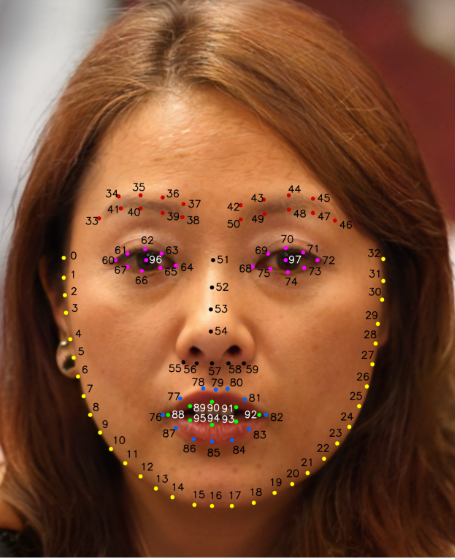
\includegraphics[width=.6\linewidth]{figures/landmark-face.png}
    \caption{Immagine dei landmark estratti dalla rete ADNet}
    \label{fig:landmark-face}
\end{figure}
\begin{itemize}
    \item dal 60 al 67: contorno occhio sinistro
    \item dal 68 al 75: contorno occhio destro
    \item 96: pupilla occhio sinistro
    \item 97: pupilla occhio destro
\end{itemize}

\section{Implementazione della metrica}
\subsection{Descrizione dell'algoritmo}
Viene inizialmente effettuata la segmentazione dell'occhio, l'algoritmo inizia isolando l'area dell'occhio dall'immagine completa utilizzando i landmarks forniti.
Una volta estratta la regione dell'occhio, l'algoritmo crea una maschera specifica per l'iride, escludendo sia la pupilla centrale (che appare normalmente scura) sia le aree esterne all'occhio. Questa segmentazione geometrica si basa su proporzioni anatomiche standard.
Lo scopo dell'algoritmo è ora quello di rilevare le zone dell'iride dove sono presenti pixel rosse, per eseguire questo compito è necessario convertire l'immagine dal tradizionale spazio colori RGB ad alcuni più utili all'isolamento di determinati colori all'interno dell'immagine quali : \begin{itemize}
    \item HSV: separa il colore dalla luminosità rendendo la misurazione meno sensibilile alle variazioni di luce
    \item yCbCr: separa luminanza da crominanza garantendo una misurazione più robusta a luce ed combre, inoltre, come illustrato dal paper "Face Detection in Color Images", questo spazio colore è ottimo per segmentare elementi facciali contraddistinti dal colore rosso.
\end{itemize}
Nel caso dello spazio colori HSV viene scelta una soglia di identificazione del colore rosso su tutti e tre i calanli.
Nel caso dello spazio colori yCbCr viene scelta una soglia minima per il canale cr, una massima per il canale cb ed inoltre vengono selezionati solamente i pixel con un valore di cr superiore alla medie per evitare problemi di saturazione.
In entrambi i casi le soglie sono state scelte in maniera sperimentale, cercando di rispettare un giosto connubio tra falsi positivi e falsi negativi.
Infine l'algoritmo calcola il rapporto tra i pixel rossi rilevati nell'iride e l'area totale dell'iride stessa, fornendo un valore normalizzato tra 0 e 1 che quantifica l'intensità dell'effetto occhi rossi.
La soglia di rosso è stata scelta in base ai risultati dei test, cercando di avere un giusto equilibrio tra falsi positivi e falsi negativi, come ad esempio le persone con gli occhi marrone o marrone chiaro.
\subsection{Dati di Input}
\begin{itemize}
    \item immagine: immagine digitale a colori
    \item puntiOcchio: vettore di punti che definiscono il contorno dell'occhio
    \item cornea: punto centrale della cornea
\end{itemize}
\subsection{Dati di Output}
\begin{itemize}
    \item rapportoRosso: valore decimale tra 0 e 1 che rappresenta la proporzione di pixel rossi nell'iride
\end{itemize}
\subsection{Algoritmo}
\begin{enumerate}
    \item Creazione maschera occhio [Fig. eye mask] \begin{itemize}
        \item Crea una maschera nera delle dimensioni dell'immagine
        \item Riempie l'area delimitata dai punti dell'occhio con bianco
        \item Calcola il rettangolo che racchiude l'occhio
    \end{itemize}
    \item Estrazione regione di interesse (ROI) \begin{itemize}
        \item Estrae la porzione di immagine corrispondente al rettangolo dell'occhio [Fig. eye roi]
        \item Estrae anche la corrispondente porzione di maschera dell'occhio [Fig. eye mask roi]
    \end{itemize}
    \item Calcolo parametri geometrici \begin{itemize}
        \item Calcola raggio pupilla = max(2, min(larghezza, altezza) / 8)
        \item Calcola raggio iride = altezza / 2
        \item Calcola centro pupilla rispetto alla ROI
    \end{itemize}
    \item Creazione maschera iride [Fig. iris mask] \begin{itemize}
        \item Crea maschera nera delle dimensioni della ROI
        \item Disegna cerchio bianco con raggio iride centrato sulla pupilla
        \item Disegna cerchio nero con raggio pupilla per escludere la pupilla centrale
    \end{itemize}
    \item Combinazione maschere [Fig. combined mask] \begin{itemize}
        \item Combina maschera occhio e maschera iride con operazione AND
        \item Risultato: maschera che isola solo la regione dell'iride
    \end{itemize}
    \item Rilevamento colore rosso [Fig. red mask] 
    \begin{itemize}
        \item Versione con HSV
            \begin{itemize}
                \item Converte l'immagine dell'occhio da BGR a HSV per migliore rilevamento colori
                \item Definisce soglie HSV per il colore rosso: \begin{itemize}
                    \item Gamma 1: H(0-10), S(100-255), V(50-255)
                    \item Gamma 2: H(160-180), S(100-255), V(50-255)
                \end{itemize}
                \item Crea maschere separate per ciascuna gamma
                \item Combina le maschere rosse con operazione OR
            \end{itemize}
        \item Versione con yCbCr
            \begin{itemize}
                \item Converte l'immagine dell'occhio da BGR a yCbCr
                \item Separa i canali cb e cr
                \item calcola media cr = la media dei valori della matrice cr
                \item calcola la matrice valoriAltiCr = maschera sui valori di cr maggiori di 150
                \item calcola la matrice valoriBassiCb = maschera sui valori di cb minori di 120
                \item calcola la matrice valoriMaggioreMediaCr = maschera sui valori di cr maggiori alla media cr
                \item calcola red mask = end logico bit a bit tra valoriAltiCr, valoriBassiCb, valoriMaggioreMediaCr
            \end{itemize}
    \end{itemize}
    \item Isolamento pixel rossi nell'iride [Fig. red iris mask] \begin{itemize}
        \item Applica maschera rossa alla maschera iride combinata
        \item Risultato: pixel rossi presenti solo nell'area dell'iride
    \end{itemize}
    \item Calcolo rapporto finale \begin{itemize}
        \item Conta pixel rossi nell'iride
        \item Conta pixel totali nell'area iride
        \item Se area iride $<$ 0: rapportoRosso = pixelRossi / pixelTotaliIride
        \item Altrimenti: rapportoRosso = 0
    \end{itemize}
    \item Ritorna rapportoRosso
\end{enumerate}
\begin{figure}
    \centering
    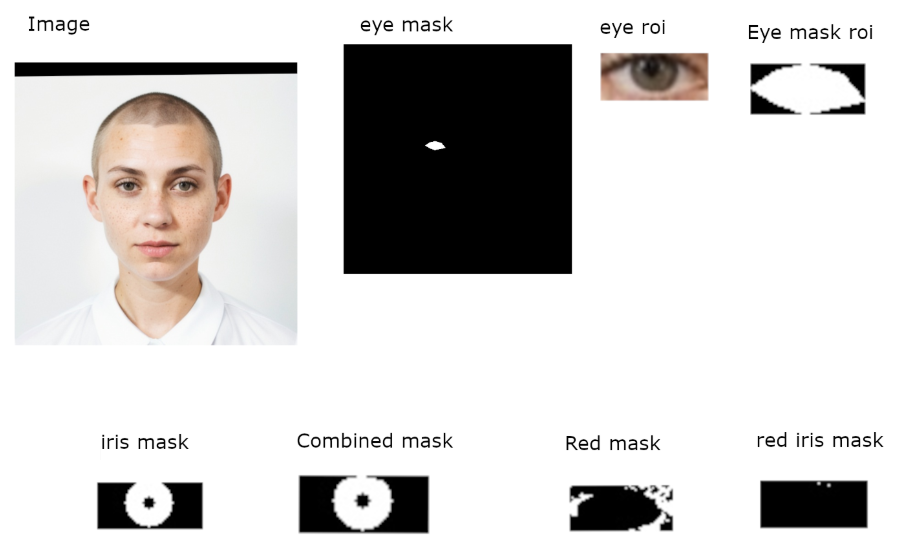
\includegraphics[width=1\linewidth]{figures/red-eye-process.png}
    \caption{Immagine descrittiva del procedimento per il rilevamento del difetto degli occhi rossi}
    \label{fig:red-eye-process}
\end{figure}

\chapter{Implementazione della metrica per il rilevamento dello sguardo frontale}

\section{Obbiettivo della metrica}
L’obiettivo della metrica è quello di assegnare uno score da 0 a 100 sul grado in cui un soggetto guarda in camera misura necessaria per garantire l’idoneità delle foto nei documenti di identità. Guardare dritto in camera è un requisito fondamentale per il riconoscimento facciale e per la conformità agli standard internazionali. 

\section{Requisiti preliminari}
I requisiti preliminari di questo task sono i landmark del viso. Il draft della ISO utilizza come riferimento per l'estrazione dei landmark facciali la CNN \href{https://github.com/huangyangyu/ADNet}{ADNet} allenata sul Wild dataset, prende in input un'immagine RGB e restituisce in output un set di 98 landmark \cref{fig:landmark-face}. I landmark che interessano questa metrica sono i seguenti:
\begin{itemize}
    \item 60, 64: angoli occhio sinistro
    \item 68, 72: angoli occhio destro
    \item 96: pupilla occhio sinistro
    \item 97: pupilla occhio destro
\end{itemize}

\section{Implementazione della metrica}


\subsection{Descrizione dell'algoritmo}
L'algoritmo analizza la direzione dello sguardo misurando la posizione delle pupille all'interno degli occhi. Per ogni occhio, calcola la larghezza totale (distanza tra gli angoli interno ed esterno) e la distanza tra la pupilla e l'angolo interno. Dividendo queste due misure ottiene un rapporto che indica dove si trova la pupilla: un valore di 0.5 significa che la pupilla è perfettamente centrata, mentre valori minori o maggiori indicano sguardo verso sinistra o destra. L'algoritmo confronta entrambi gli occhi e sceglie quello con maggiore deviazione dal centro per determinare la direzione principale dello sguardo. Infine, applica una trasformazione parabolica (con parametri alpha = -400 e beta = 100) che mappa il risultato su una scala da 0 a 100, dove valori più alti indicano maggiore deviazione dalla posizione frontale. Questo approccio permette di quantificare oggettivamente quanto una persona stia guardando lateralmente rispetto alla fotocamera.
Una visione grafica dei rapporti sopra elencati è disponibile 

\begin{figure}
    \centering
    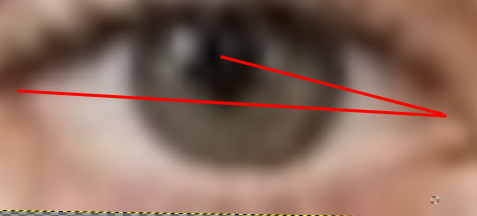
\includegraphics[width=.4\linewidth]{figures/frontal_gaze_manual.png}
    \caption{Immagine rappresentativa dei rapporti utilizzato dall'algoritmo di stima dello sguardo frontale manuale}
    \label{fig:frontal-gaze-manual}
\end{figure}

\subsection{Dati di Input}
\begin{itemize}
    \item a: coordinate x ed y dell'angolo esterno dell'occhio sinistro
    \item b: coordinate x ed y dell'angolo interno dell'occhio sinistro
    \item c: coordinate x ed y dell'angolo esterno dell'occhio destro
    \item d: coordinate x ed y dell'angolo interno dell'occhio destro
    \item e: coordinate x ed y della pupilla dell'occhio sinistro
    \item f: coordinate x ed y della pupilla dell'occhio destro
\end{itemize}
\subsection{Dati di Output}
\begin{itemize}
    \item valoreScalare: valore numerico che rappresenta la deviazione dello sguardo da 0 a 100
\end{itemize}
\subsection{Algoritmo}
\begin{enumerate}
    \item Calcolo larghezza degli occhi \begin{itemize}
        \item \(larghezzaSinistra = \sqrt{(b_x - a_x)^2 + (b_y - a_y)^2}\)
        \item \(larghezzaDestra = \sqrt{(d_x - c_x)^2 + (d_y - c_y)^2}\)
    \end{itemize}
    \item Calcolo distanza pupilla-angolo interno \begin{itemize}
        \item \(distanzaSinistra = \sqrt{(e_x - b_x)^2 + (e_y - b_y)^2}\)
        \item \(distanzaDestra = \sqrt{(f_x - d_x)^2 + (f_y - d_y)^2}\)
    \end{itemize}
    \item Calcolo rapporti normalizzati \begin{itemize}
        \item \(rapportoSinistro = \frac{distanzaSinistra}{larghezzaSinistra}\)
        \item \(rapportoDestro = \frac{distanzaDestra}{larghezzaDestra}\)
    \end{itemize}
    \item Calcolo variazioni dal centro (\textit{Nota: 0.5 rappresenta la posizione centrale ideale della pupilla}) \begin{itemize}
        \item \(variazioneSinistra = |rapportoSinistro - 0.5| \)
        \item \(variazioneDestra = |rapportoDestro - 0.5| \)
    \end{itemize}
    \item Selezione rapporto dominante \begin{itemize}
        \item Se \(variazioneDestra > variazioneDestra \) allora: \(punteggioGrezzo = rapportoSinistro \)
        \item Altrimenti: \(punteggioGrezzo = rapportoDestro\)
    \end{itemize}
    \item Applicazione funzione di scaling \begin{itemize}
        \item \(alpha = -400\)
        \item \(beta = 100 \)
        \item Calcola \(valoreScalare = alpha \cdot (punteggioGrezzo - \frac{1}{2})^2 + beta\)
    \end{itemize}
\end{enumerate}

\chapter{Rilevamento dello sguardo frontale tramite CNN}
\subsection{Selta del modello}
Dopo un'attenta analisi sui modelli stato dell'arte nel task del rilevamento dello sguardo si è trovato come riferimento l'implementazione della rete neurale descritta all'interno del paper \cite[L2CS-NET: FINE-GRAINED GAZE ESTIMATION IN UNCONSTRAINED ENVIRONMENTS]{10372944}.
Il modello descritto in questo paper si propone di prevedere lo sguardo in ambienti non vincolati, dando una stima degli angoli Pitch e Yaw del volto in radianti.

\subsection{Utilizzo del modello}
Il modello L2CS-NET viene distribuito sotto forma di pacchetto Python.
Il pacchetto espone un API tramite la quale è possibile far processare un'immagine ed ottenere per ogni volto dell'immagine gli angoli Pitch e Yaw.
Il modello L2CS-NET è costruito mediante il framework Pytorch ed è quindi un modello Pytorch, per poter utilizzare il modello all'interno del software OFIQ è necessario covnertire il modello al formato Onnx, un formato open utilizzato per rappresentare i modelli di machine learning.
Il formato Onnx permettere di eseguire il modello all'interno del software OFIQ in C++ tramite la libreria OnnxRuntime disponibile in C++.
Inoltre il pacchetto Python di L2CS-NET esegue il preprocessa dell'immagine tramite una pipeline che effettua i sueguenti step: \begin{itemize}
    \item Utilizza il modello RetinaFace (dalla libreria face detection) per trovare il bounding box dei vari volti all'interno dell'immagine
    \item Per ogni volto viene presa in considerazione solamente la parte dell'immagine compresa all'interno della bounding box (regione di interesse)
    \item Per ogni regione di interesse viene convertito lo spazio colori da BGR a RGB
    \item Ogni regione di interesse viene ridimensionato in un'immagine (224 * 224)
    \item Ogni regione di interesse viene passata al modello ResNet-50 seguito da 2 layer fully-connected che ritornano in output 90 classi rappresentanti intervalli discreti (sia per pitch che per yaw) con all'interno un valore rappresentante la probabilità che lo sguardo per il relativo angolo si trovi in quell'intervallo
    \item Per ogni valore ritornato da ResNet-50 viene applicata la funzione Softmax di modo da avere la probabilità in percentuale che lo sguardo si trovi all'interno di quell'intervallo
    \item Vengono moltiplicate le probabilità che lo sguardo si trovi in quell'intervallo per l'indice della probabilità nel vettore dei tensori
    \item Viene fatta la somma dei valori ottenuti precedentemente
    \item La somma viene moltiplicata per quattro ed il risultato sottratto di 180, in modo da convertire ogni probabilità ottenuta gradi.
    \item Viene eseguita la conversione da gradi a radianti
\end{itemize}
I passaggi che includono l'utilizzo di open cv sono facilmente replicabili all'interno del software OFIQ tramite la libreria open cv per cpp, mentre per trovare il bounding box del volto all'interno dell'immagine viene utilizzato il modello "SSD Face Detector CNN" che riporta risultati molto simili a quelli di RetinaFace, la scelta di utilizzare questo modello è dettata dal fatto di averlo già a disposizione all'interno del software in formato Onnx.

\subsection{Implementazione della metrica}

\subsection{Dati di Input}
\begin{itemize}
    \item immagine: L'immagine del volto da valutare
\end{itemize}
\subsection{Dati di Output}
\begin{itemize}
    \item valoreScalare: valore numerico che rappresenta la deviazione dello sguardo da 0 a 100
\end{itemize}
\subsection{Algoritmo}
\begin{enumerate}
    \item Calcola \(detectedFaces\) tramite il modello SSD Face Detector CNN
    \item Se \(detectedFaces.length < 1\) allora: \(valoreScalare = 0\). Fine.
    \item \(faceBoundingBox = detectedFaces[0]\), solamente il primo volto trovato verrà valutato
    \item Carica il modello in formato onnx tramite onnxRuntime
    \item Calcola \(immagineVolto\) = la sezione di immagine all'interno di \(faceBoundingBox\)
    \item Preprocessing per L2CS-NET \begin{itemize}
        \item Definisce \(inputSize = 443\)
        \item Calcola \(immagineRidimensionata\) ridimensionando con open cv \(immagineVolto\) alla grandezza (\(inputSize\) x \(inputSize\))
        \item Converte lo schema colore di \(immagineRidimensionata\) da BGR a RGB
        \item Scala i valori dell'immagine dall'intervallo [0,255] a [0,1] convertendoli a float
        \item Normalizza l'immagine \begin{itemize}
            \item Definisce \(mean = [0.485f, 0.456f, 0.406f]\) (dal preprocessing della librerie L2CS-NET)
            \item Definisce \(std = [0.229f, 0.224f, 0.225f]\) (dal preprocessing della librerie L2CS-NET)
            \item Per ogni canale RGB dell'immagine: \(channels[i] = \frac{(channels[i] - mean[i])}{std[i]}\) con \(i = 0..3\)
            \item Definisce \(immaginePreprocessata\) la matrice formata dai canali normalizzati nei punti precedenti
        \end{itemize}
        \item Definisce \(input_shape = [1, 3, inputSize, inputSize]\) (aggiunge la dimensione della batch (in questo caso 1 dato che viene processata solamente un'immagine))
        \item Converte l'input in una matrice CHW: \begin{itemize}
            \item Per ogni canale \(c = 0..3\): 
            \item Per ogni riga dell'immagine \(h = 0...inputSize\) 
            \item Per ogni colonna dell'immagine \(w = 0...inputSize\) 
            \item \(tensoreInput[c * inputSize * inputSize + h * inputSize + w] = immaginePreprocessata[h][w][c]\)
        \end{itemize}
    \end{itemize}
    \item Vengono usate le API offerte da \(onnxRuntime\) per eseguire il modello L2CS in formato Onnx. 
    \item Vengono calcolati \(pitch\) e \(yaw\) sulla base dell'output del modello (il modello restituisce in output i valori per 90 classi sia per pitch che per yaw, i seguenti step vengono eseguiti per entrambi gli angoli) 
    \item \begin{itemize} 
        \item Sia \(x\) il vettore con i 90 valori
        \item \(angoloInRadianti = \frac{\sum_{i}^{x} (e^{x_i}*i)}{\sum_i^{x}(e^x)}\) * 4 - 180
    \end{itemize}
    \item \( value = max(|pitch|, |yaw|) \) (Si usa il valore assoluto in quanto lo sguardo frontale viene classificato come angolo 0)
    \item \( score = round((1 - (\frac{min(value, 45)}{45}))*100) \) (Uso 45 come valore limite, tutti valore da 45 a 180 vengono classificati come punteggio 0)
    \item value è il valore assoluto dell'angolo più lontano da 0 Gradi, mentre score è la valutazione dell'immagine da 0 a 100
\end{enumerate}

\chapter{Strumenti utilizzati per lo sviluppo delle metriche}
\section{Software OFIQ}
Il software OFIQ, acronimo di Open Source Face Image Quality, è un software open source sviluppato per implementare le metriche descritte nel draft dello standard ISO 29794-5.
Il software è scritto in linguaggio C++ e dispone di CMake file per la compilazione su sistemi Linux, Windows e MacOS.
Il software al suo interno utilizza librerie quali OpenCV per la gestione delle immagini ed OnnxRuntime per l'esecuzione dei modelli Onnx.
Il software inizialmente presentava un'implementazione fedele di tutte le metriche presentati nello standard ISO 29794-5 restituendo in output un valore per ogni metrica grezzo ed un valore normalizzato tra 0 e 100 (utile come score).
Il software OFIQ al suo interno contiene delle utility che permettono l'utilizzo dei seguenti modelli (presenti in formato Onnx): \begin{itemize}
    \item SSD Face Detector CNN: modello per il rilevamento dei volti all'interno di un'immagine.
    \item ADNet: Modello per l'estrazione dei landmark facciali.
\end{itemize}
Il software presenta l'implementazione delle seguenti metriche: \begin{itemize}
    \item Quality Score: uno score generale dell'immagine ottenuto tramite l'utilizzo del modello MagFace..
    \item Background uniformity: misura l'uniformità del background.
    \item Illumination uniformity: misura l'uniformità di illuminazione eseguendo il rapporto tra l'illuminazione della parte destra e sinistra del volto.
    \item Luminance mean: verifica che l'immagine abbia un'illuminazione adeguata e uniforme.
    \item Luminance variance: misura i constasti nell'immagine.
    \item Under-exposure prevention: verifica che l'immagine abbia troppi pixel con una bassa luminosità.
    \item Over-exposure prevention:  verifica che l'immagine abbia troppi pixel con un'alta luminosità.
    \item Dynamic range: misura quanta variazione di intensità luminosa è presente nella regione del volto, assicurandosi che non sia tutta troppo scura o troppo chiara.
    \item Sharpness: valuta la nitidezza di un'immagine (la corretta messa a fuoco).
    \item No compression artifacts: valuta la presenza di artefatti di compressione, assicurandosi che l'immagine non sia stata eccessivamente compressa.
    \item Natural colour: valuta la naturalezza del colore della pelle in un'immagine del volto.
    \item Single face present: valuta la presenza di un singolo volto nell'immagine.
    \item Eyes open: verifica che entrambi gli occhi siano aperti in maniera naturale.
    \item Mouth closed: verifica che la bocca sia chiusa.
    \item Eyes visible: verifica che in entrambi gli occhi sia visibile pupilla ed iride.
    \item Mouth occlusion prevention: verifica la non occlusione della bocca
    \item Face occlusion prevention: verifica che la regione del viso dalla sommità del capo alla base del mento e da un orecchio all'altro, sia chiaramente visibile.
    \item Inter-eye distance: verifica in pixel la distanza tra gli occhi nel volto
    \item Head size: valuta la dimensione del volto nell'immagine per evitare volti troppo vicini alla telecamera
    \item Leftward crop of face in image: verifica che il volto non sia decentrato sulla sinistra.
    \item RIghtward crop of face in image: verifica che il volto non sia decentrato sulla destra.
    \item Downward crop of face in image: verifica che il volto non sia decentrato in basso.
    \item Upward crop of face in image: verifica che il volto non sia decentrato in alto.
    \item Pose angle yaw frontal alignment: verifica che l'angolo yaw del volto sia minore di \(\pm 5\) dal frontale.
    \item Pose angle pitch frontal alignment: verifica che l'angolo pitch del volto sia minore di \(\pm 5\) dal frontale.
    \item Pose angle roll frontal alignment: verifica che l'angolo roll del volto sia minore di \(\pm 8\) dal frontale.
    \item Expression neutrality: verifica che la faccia abbia un'espressione neutrale.
    \item No head covering: verifica che il soggetto non stia indossando qualcosa che copra la testa (eg un cappello).
\end{itemize}

\section{Dataset utilizzati per la valutazione}
I seguenti dataset sono stati utilizzati per valutare la valutazione delle metriche implementate.
\subsection{ONOT}
ONOT è un dataset introdotto nel paper \cite[ONOT: a High-Quality ICAO-compliant Synthetic Mugshot Dataset]{di2024onot}.
Si tratta di un dataset composto da immagini sintetiche di alta qualità conformi ai requisiti delllo standard ISO/IEC 39794-5.
Definisce un formato di per lo scambio di immagini facciali in electronic Machine-Readable Travel Documents (eMRTD), seguendo le linee guida del International Civil Aviation Organization (ICAO).
Le immagini presenti in questo dataset presentano volti di diverse etnie, età, genere e tratti facciali, rendendo questo dataset perfetto per testare le metriche implementate.
Del dataset TONO sono state prese le sole immagini del \textit{Subset 1} ICAO compliant.

\subsection{TONO}
TONO è un dataset introdotto nel paper \cite[TONO: a synthetic dataset for face image compliance to ISO/ICAO standard]{borghi2024tono}.
Si tratta di un dataset composto da immagini sintetiche di volti di alta qualità costruito per sviluppare e valutare sistemi volti a verificare la conformità in un immagine di un volto allo standard ISO/ICAO.
Le immagini di Tono sono state create partendo dal dataset ONOT (\cite{di2024onot}) con uno o più elementi non conformi allo standard ISO/ICAO.
I difetti presenti in TONO sono i seguenti: \begin{itemize}
    \item Head and Shoulder Pose: assenza di posa frontal sia del volto che delle spalle.
    \item Gaze Direction: assenza di sguardo frontale.
    \item Expression: assenza di espressione neutrale o denti visibili.
    \item Face Illumination: assenza di uniformità nell'illuminazione del volto.
    \item Background: background non uniforme.
    \item Head Coverings: presenza di copri capo.
    \item Eye Visibility: presenza di occhi chiusi con e senza occhiali, mackeup troppo presente, presenza di occhiali da sole.
    \item Photographic: presenza dei difetti di: pixelazione, posterizzazione, sfocato, sovraesposizione, sovrasaturazione.
\end{itemize}

\section{Onnx e OnnxRuntime}
ONNX (Open Neural Network Exchange) è un formato open source per rappresentare modelli di machine learning, progettato per essere compatibile tra diversi framework (PyTorch, TensorFlow, etc.).
Permette di salvare un modello in un file .onnx indipendente dall'ambiente di training.
La libreria Onnx Runtime predispone API per essere utilizzata da diversi linguaggi di programmazione e su diverse piattaforme (tra cui i web browser).
Il progetto nasce da Microsoft ed il sorgente è disponibile alla seguente reporitory github: \href{https://github.com/microsoft/onnxruntime}{https://github.com/microsoft/onnxruntime}.

\section{FVC Ongoing}
FVC Ongoing (\cite{fvcongoing}) è una piattaforma web che permette di valutare algoritmi di vario tipo tra cui il task Face Image ISO Compliance Verification, I test vengono effettuati tramite diversi dataset e metriche note.

\section{Framework Pytorch}
Il linguaggio di programmazione Python ed il framework Pytorch sono comunemente utilizzati per l'addestramento e la distribuzione di modelli di Machine Learning. Il loro impiego all'interno del progetto è relativo al testing ed alla conversione in formato onnx del modello L2CS-Net, distribuito come modello Pytorch.
Del framework Pytorch è stato utilizziato in particolare il modulo "ONNX exporter API" che permette di esportare un modello Pytorch in formato Onnx, utilizzato per la conversione di L2CS-Net tramite il seguente codice: \cref{lst:onnx-exporter}

\lstinputlisting[float,language=Python,label={lst:onnx-exporter}]{listings/onnx_exporter.py}

\section{Jupyter Notebook, Numpy e Matplotlib}
Jupyter Notebook, Numpy e MatplotLib sono state utilizzati per creare documenti interattivi per mostrare sotto forma di grafici boxplot e istogrammi le performance delle metriche di valutazione sui dataset disponibili, in questo caso Onot, Tono ed un sottoinsieme di Biolab.
Il linguaggio python è stato utilizzato anche per task quali \begin{itemize}
    \item Divisione dei dataset in base al file txt di riferimento
    \item Elaborazione delle metriche volte a valutare il software OFIQ e gli algoritmi proposti
\end{itemize}

\chapter{Valutazione delle metriche}

\section{Valutazione su FVC-Ongoing}

\subsection{Metriche valutate}
La piattaforma FVC-Ongoing valuta le seguenti 24 diverse metriche \cref{tab:fvc-table}.
Nel caso di questo progetto le metriche da valutare sarranno \begin{itemize}
    \item Looking Away: valuta se un soggetto sta guardando in camera
    \item Red Eyes: Valuta se un soggetto ha il difetto degli occhi rossi
\end{itemize}
\begin{table}[h!]
\centering
\begin{tabular}{|c|p{8cm}|c|}
\hline
\textbf{N°} & \textbf{Description of the test}  \\
\hline
\multicolumn{2}{|l|}{\textbf{Feature extraction accuracy tests}} \\
1 & Eye center location accuracy \\
\hline
\multicolumn{2}{|l|}{\textbf{Photographic and pose-specific tests}} \\
2 & Blurred \\
3 & Looking away \\
4 & Ink marked/creased \\
5 & Unnatural skin tone \\
6 & Too dark/light \\
7 & Washed out \\
8 & Pixelation \\
9 & Hair across eyes \\
10 & Eyes closed \\
11 & Varied background \\
12 & Roll/pitch/yaw > predefined thresholds \\
13 & Flash reflection on skin \\
14 & Red eyes \\
15 & Shadows behind head \\
16 & Shadows across face \\
17 & Dark tinted lenses \\
18 & Flash reflection on lenses \\
19 & Frames too heavy \\
20 & Frame covering eyes \\
21 & Hat/cap \\
22 & Veil over face \\
23 & Mouth open \\
24 & Other faces/toys too close \\
\hline
\end{tabular}
\caption{Metriche valutate da FVC-Ongoing}
\label{tab:fvc-table}
\end{table}

\subsection{Il protocollo}
Per la sottomissione degli algoritmi sulla piattaforma FVC-Ongoing è necessario rispettare il seguente standard: \begin{itemize}
    \item è necessario sottoporre una cartella in formato ZIP
    \item All'interno della cartella deve essere presente un file \textit{Check.exe} che un eseguibile per Win 32 in formato console application
    \item la sintassi a linea di comando deve essere la seguente: "./Check.exe $<$faceimagefile$>$ $<$outputfile$>$" dove \begin{itemize}
        \item faceimagefile: è il percorso dell'immagine del volto da valutare e può essere in formato BPM, JPG, PNG
        \item outputfile: è il percorso del file TXT di output dove dovrà essere scritta in modalità 'append' una stringa rappresentante l'esito dei test
    \end{itemize}
    \item Ogni linea del outputfile dovrà contenere i campi seguenti separati da uno spazio vuoto: \begin{itemize}
        \item ImageName: il nome file dell'immagine
        \item RetVal: 
    \end{itemize}
\end{itemize}

\chapter{State of the art}

I suggest referencing stuff as follows: \cref{fig:random-image} or \Cref{fig:random-image}

\begin{figure}
    \centering
    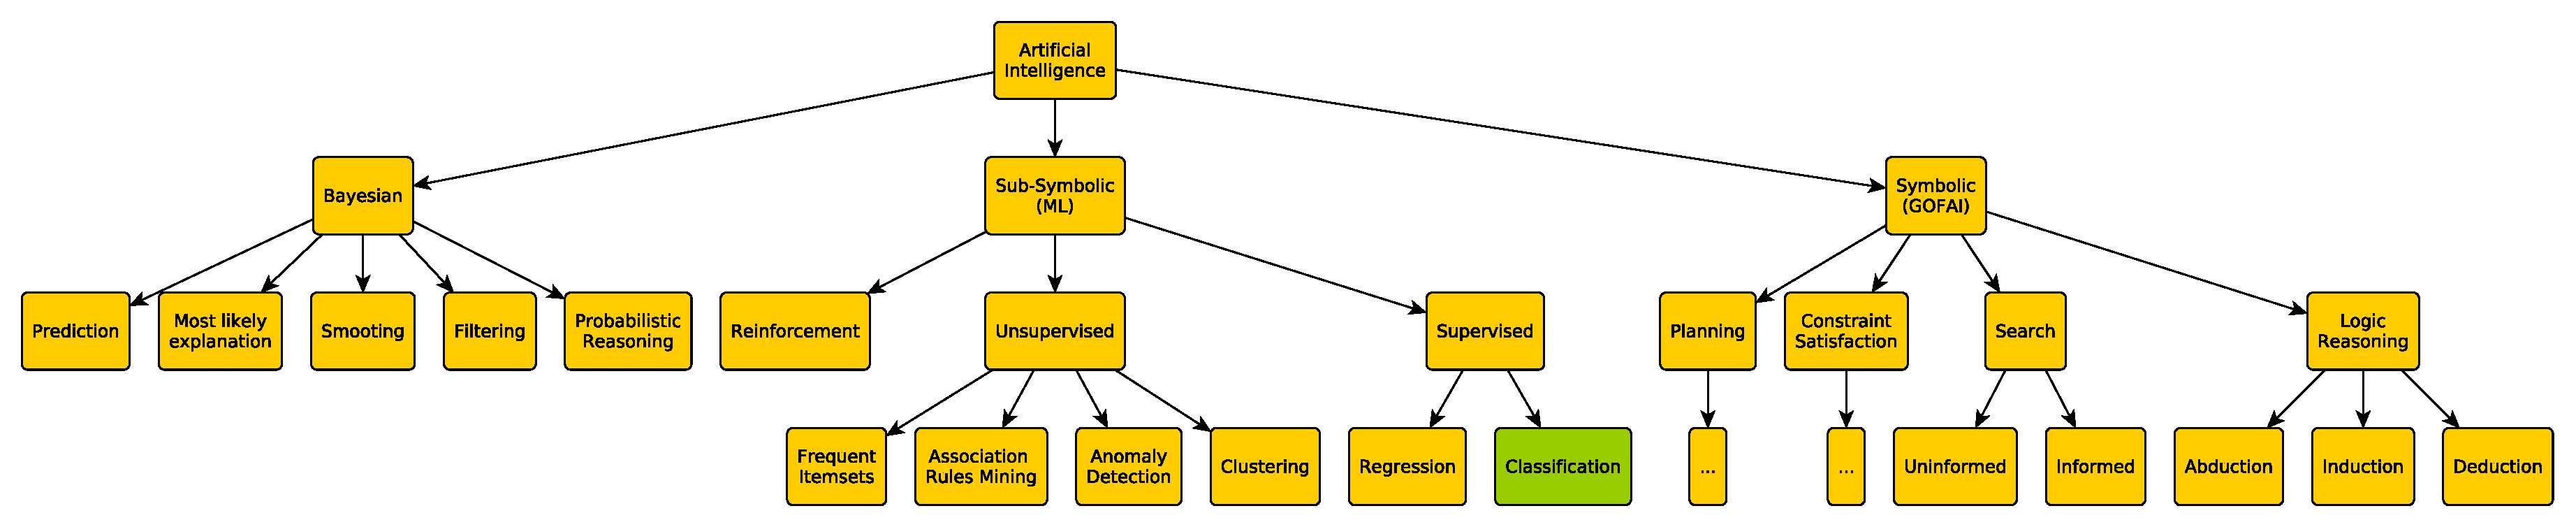
\includegraphics[width=.8\linewidth]{figures/random-image.pdf}
    \caption{Some random image}
    \label{fig:random-image}
\end{figure}

\section{Some cool topic}

\chapter{Contribution}


\section{Fancy formulas here}

%----------------------------------------------------------------------------------------
% BIBLIOGRAPHY
%----------------------------------------------------------------------------------------

\backmatter

\nocite{*} % Remove this as soon as you have the first citation

\bibliographystyle{alpha}
\bibliography{bibliography}



\begin{acknowledgements} % this is optional
Optional. Max 1 page.
\end{acknowledgements}

\end{document}
